\documentclass[12pt,letterpaper]{exam}
\usepackage[lmargin=1in,rmargin=1in,tmargin=1in,bmargin=1in]{geometry}
\usepackage{../style/exams}

% -------------------
% Course & Exam Information
% -------------------
\newcommand{\course}{MAT 108: Exam 1}
\renewcommand{\term}{Fall -- 2023}
\newcommand{\examdate}{10/03/2023}
\newcommand{\timelimit}{85 Minutes}

\setbool{hideans}{false} % Student: True; Instructor: False

% -------------------
% Content
% -------------------
\begin{document}

\examtitle
\instructions{Write your name on the appropriate line on the exam cover sheet. This exam contains \numpages\ pages (including this cover page) and \numquestions\ questions. Check that you have every page of the exam. Answer the questions in the spaces provided on the question sheets. Be sure to answer every part of each question and show all your work. If you run out of room for an answer, continue on the back of the page --- being sure to indicate the problem number.} 
\scores
\bottomline
\newpage

% ---------
% Questions
% ---------
\begin{questions}

% Question 1
\newpage
\question[10] Suppose that the current CPI is 307.026. Further, suppose that the CPI next year at this time will be 319.307. 
	\begin{enumerate}[(a)]
	\item Find the inflation rate from this year to next year. 
	\item Estimate the cost of a good next year that currently costs \$29.99. 
	\item If this inflation rate continue across the next decade, what will be percentage increase in costs ten years from now compared to now?
	\end{enumerate} \pspace

\sol 
\begin{enumerate}[(a)]
\item If $r$ was the inflation rate, then $319.307= 307.025(1 + r)$; equivalently, $1 + r= \frac{319.307}{307.026}$. We know\dots
	\[
	\dfrac{319.307}{307.026}= 1.04= 1 + 0.04
	\]
But then $1 + r= 1 + 0.04$, which implies $r= 0.04$. Therefore, the inflation rate from this year to next year is $4\%$. \pspace

\item If we want to compute $N$ increased or decreased by a \%, we compute $N \cdot (1 \pm \%_d)$, where $\%_d$ is the percentage written as a decimal and we choose `$+$' if it is a percentage increase and choose `$-$' if it is a percentage decrease. From (a), we know that the inflation rate is 4\%. But then the cost of the good should increase by 4\% by next year. Therefore, the price should be\dots
	\[
	N \cdot (1 \pm \%_d)= \$29.99(1 + 0.04)= \$29.99(1.04)= \$31.1896 \approx \$31.19
	\] \pspace

\item If we want to compute $N$ repeatedly increased or decreased by a \% a total of $n$ times, we compute $N(1 \pm \%_d)^n$, where $\%_d$ is the percentage written as a decimal, and we choose `$+$' if it is a repeated percentage increase and `$-$' if it is a repeated percentage decrease. But then if the price of a good, $P$, increased by 4\% every year for 10~years, the final price would be\dots
	\[
	N(1 \pm \%_d)^n= P (1 + 0.04)^{10}= P(1.04)^{10}= P(1.4802443)= P(1 + 0.4802443)
	\]
Therefore, if the inflation rate continues to be 4\% each year for the next decade, then the prices a decade from now will be 48.02\% higher. 
\end{enumerate}

\vfill

{\scriptsize\itshape Note. For (c), observe that this percentage increase is the same---independent of the initial cost of the good. So one may use any good price to find this percentage increase. Suppose a good costs \$100. We will find the percentage increase in the cost of this good after a decade of inflation: $\$100(1 + 0.04)^{10}= 148.02443$. But from this, it is immediately clear that prices in a decade will be 48.02443\% higher.}



% Question 2
\newpage
\question[15] Consider the revenue function, $R(q)$, and cost function, $C(q)$, for some good given in the plot below. 
	\[
	\fbox{
	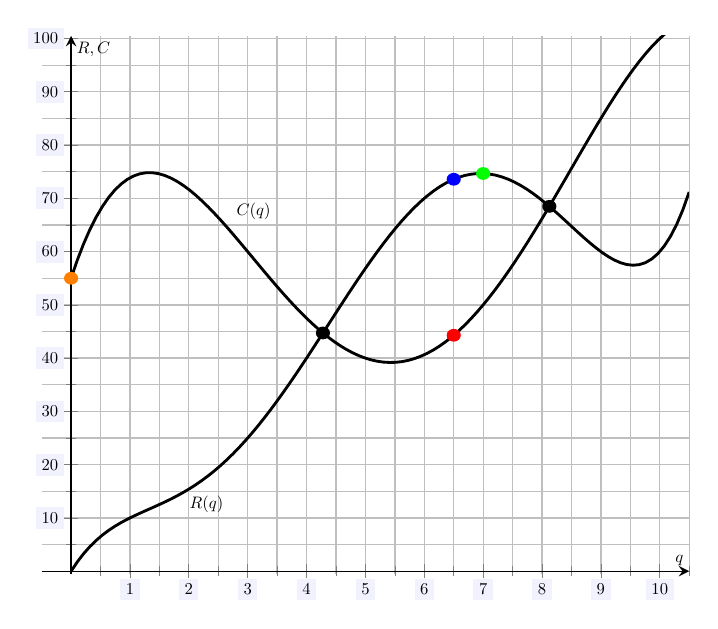
\begin{tikzpicture}[scale=1.2,every node/.style={scale=0.5}]
	\begin{axis}[
	grid=both,
	axis lines=middle,
	ticklabel style={fill=blue!5!white},
	xmin= -0.5, xmax=10.5,
	ymin= -0.5, ymax=100.5,
	xtick={0,1,2,...,11},
	ytick={0,10,20,...,100},
	minor x tick num = 1,
	minor y tick num = 1,
	xlabel=\(q\),ylabel=\({R,C}\),
	]
	\node at (2.3,12.5) {$R(q)$};
	\addplot[domain=0:10.5, samples=100,line width=0.03cm] 
	(x, 17.6667*x - 11.3056*x^2 + 4.16204*x^3 - 0.546296*x^4 + 0.0231481*x^5);
	\node at (3.1,67.5) {$C(q)$};
	\addplot[domain=0:10.5, samples=100,line width=0.03cm] 
	(x, 55 + 33.994*x - 17.7014*x^2 + 2.69544*x^3 - 0.131944*x^4 + 0.000992063*x^5);
	
	\draw[fill=orange,draw=none] (0,55) ellipse (0.12 and 1.2);
	
	\draw[fill=black,draw=none] (4.2783,44.7277) ellipse (0.12 and 1.2);
	\draw[fill=black,draw=none] (8.12396,68.4927) ellipse (0.12 and 1.2);
	\draw[fill=black,draw=none] (11.0899,101.965) ellipse (0.12 and 1.2);
	
	\draw[fill=blue,draw=none] (6.5,73.5849) ellipse (0.12 and 1.2);
	\draw[fill=red,draw=none] (6.5,44.2946) ellipse (0.12 and 1.2);
	
	\draw[fill=green,draw=none] (7,74.6656) ellipse (0.12 and 1.2);
	\end{axis}
	\end{tikzpicture}
	}
	\] 
In the plot above, the number of goods produced, $q$, is measured in tens of thousands of items and the outputs of $R(q)$ and $C(q)$ are measured in tens of thousands of dollars. Given this data, answer the following:
	\begin{enumerate}[(a)]
	\item What are the fixed costs?
	\item What the break-even point(s)?
	\item Is the company experiencing profit or loss for this good at a production level of 65,000~units?
	\item Estimate the profit or loss in (c). 
	\item Estimate the average revenue per sale at a production/sale level of 70,000~units. 
	\end{enumerate} \pspace

\sol 
\begin{enumerate}[(a)]
\item The fixed costs are the cost that occur regardless of the level production of the good. In particular, these are the costs that occur when there is no production, i.e. $C(0)$. Either finding $C(0)$ on the graph or recognizing that $C(0)$ is the $y$-intercept of $C(q)$ (the orange point in the graph), we see that $C(0)= 55$~tens of thousands of dollars, i.e. the fixed costs are \$550,000. \pspace

\item A break-even point is a production level where revenue equals cost, i.e. $R(q)= C(q)$. But these are the $q$-values where $R(x)$ and $C(q)$ intersect (the black points in the graph). Examining the graph, we see that the break-even points are $q \approx 4.2783$ and $8.12396$, i.e. production levels of 42,783~units and 81,239.6~units. \pspace

\item We know that 65,000~units is a production level of 6.5~tens of thousands of units. So we need to compare $R(6.5)$ and $C(6.5)$ (the blue and red points in the graph, respectively). Examining the graph, we see that $R(6.5) > C(6.5)$, i.e. the revenue at a production level of 65,000~units is greater than the costs at that production level. Therefore, the company must be making a profit. \pspace

\item From (c), we know that the company is making a profit at a production level of 65,000 units, i.e. 6.5~tens of thousands of units. Examining the graph, we see that $R(65) \approx 73.584916$ and $C(6.5) \approx 44.294587$. We know the profit is $R(6.5) - C(6.5)= 73.584916 - 44.294587= 29.290329$~tens of thounsands of dolllars, i.e. the company makes \$292,903.29 in profit at a production level of 65,000 units. \pspace

\item A production level of 70,000 units is 7~tens of thousands of units. Therefore, we want to find $\text{Avg. R}(70)= \frac{R(70)}{70}$. Examining the graph, we see that $R(70) \approx 74.6656407$ (the green point in the graph). Therefore, $\text{Avg. R}(70)= \frac{R(70)}{7} \approx \frac{74.6656407}{7} \approx 10.6665201$, i.e. the company makes on average \$1066,65.20 per sale of tens of thousands of items---which is approximately \$10.67 per item. 
\end{enumerate}



% Question 3
\newpage
\question[15] Kriss Crosse is taking out a loan to expand her applesauce business. The bank offers her a \$260,000 loan at 14.6\% annual interest, compounded monthly. By accepting the loan terms, Ms. Crosse will pay \$30,000 up-front. The remainder of the loan will be repaid with equal, end of the month payments of \$4,074.38 over 8~years
	\begin{enumerate}[(a)]
	\item How much will Kriss still owe on the loan after 6~years of payments?
	\item How much interest will Kriss pay in total for this loan?
	\end{enumerate} \pspace

\sol Because there will be regular, equal payments for this loan, this is an amortization. Because payments are made at the end of a payment period, this is an amortization based on an ordinary annuity (or an annuity-immediate). Finally, because the number of payments per year is the same as the number of compounds per year, this amortization is based on a simple ordinary annuity (or a simple annuity-immediate). \pspace

For this amortization, we know that the initial amount of the loan is the amount after Kriss has paid the \$30,000 up-front. Therefore, the principal for the loan is $\$260000 - \$30000= \$230000$, i.e. $P= \$230000$. We know that the annual interest rate is $r= 0.146$ and is compounded monthly, i.e. $k= 12$ times per year. Because this is a simple annuity, the interest per payment period is then $i= \frac{r}{k}= \frac{0.146}{12} \approx 0.0121666666667$. Because payments are made monthly over a period of $t= 8$~years, the number of payments is $\text{PM}= \text{PY} \cdot t= 12 \cdot 8= 96$. Finally, the end of the month payments are $R= \$4074.38$. \pspace

\begin{enumerate}[(a)]
\item We need to find how much Kriss still owes after 6~years of payments, i.e. after $M= 12 \cdot 6= 72$~payments. But then there are $\text{PM} - M= 96 - 72= 24$~payments left. 

We first compute\dots
	\[
	\hspace{-1.5cm} a_{\actuarialangle{\text{PM} - \text{M}\,}\, i}= a_{\actuarialangle{24\,}\, 0.0121666666667}= \dfrac{1 - (1 + 0.0121666666667)^{-24}}{0.0121666666667}= \dfrac{0.25191445644}{0.0121666666667}= 20.70529779
	\]
But then\dots
	\[
	\text{A.O.}= R\, a_{\actuarialangle{\text{PM} - \text{M}\,}\, i}= \$4074.38 \cdot a_{\actuarialangle{24\,}\, 0.0121666666667}= \$4074.38 \cdot 20.70529779 \approx \$84,\!361.25
	\]
Therefore, after 6~years of payments, Kriss still owes \$84,361.25. \pspace

\item If Kriss makes 96~payments of \$4,074.38, then Kriss will pay\dots
	\[
	\text{Total Paid}= \text{PM} \cdot R= 96 \cdot \$4074.38= \$391,140.48
	\]
Kriss only need pay back the principal of \$230,000. Any other money Kriss pays is in interest. But then the total amount of interest Kriss pays is\dots
	\[
	I= \text{PM} \cdot R - P= \$391\!,140.48 - \$230\!,000= \$161,\!140.48
	\]
\end{enumerate}



% Question 4
\newpage
\question[15] Braden Haire is investing some of the profits from his politically active wig company Wigs for Whigs. He places \$65,000 into an account that advertises a 4.15\% annual interest rate, compounded continuously. 
	\begin{enumerate}[(a)]
	\item One year from now, by what percentage would Braden's money have increased?
	\item Assuming Braden makes no additional deposits into the account, how much will be in the account after 33~years?
	\item How much interest would the account have earned after 33~years?
	\end{enumerate} \pspace

\sol Because Braden simply deposits the money into an account and makes no further payments, withdrawals, etc., this is not an annuity but rather an `ordinary interest problem.' Because the interest is compounded continuously, this is an `ordinary compounded continuously interest problem.' \pspace

We know the initial amount that Braden deposits, i.e. the principal, into the account is $P= \$65000$. The account earns an annual interest rate of $r= 0.0415$, compounded continuously. \pspace

\begin{enumerate}[(a)]
\item This is the effective interest, which is\dots
	\[
	r_{\text{eff}}= e^r - 1= e^{0.0415} - 1= 1.0423732 - 1= 0.0423732
	\]
Therefore, after one year, Braden's initial investment would have increased by approximately 4.24\% due to the interest earned. \pspace

\item This is the future value of the initial investment, i.e. the principal, after $t= 33$~years. But this is\dots 
	\[
	F= Pe^{rt}= \$65000 e^{0.0415 \cdot 33}= \$65000 e^{1.3695}= \$65000 \cdot 3.9333835 \approx \$255,\!669.93
	\] \pspace

\item Any money in the account was either the initial amount placed in the account, i.e. the principal, or due to interest. From (b), after 33~years, we know the account has \$255,669.93. The principal was \$65,000. Therefore, the amount of interest earned was\dots
	\[
	\text{Interest Earned}= F - P= \$255,\!669.93 - \$65,\!000= \$190,\!669.93
	\]
\end{enumerate}

\vfill 

{\scriptsize\itshape Note. For (a), one can compute the future value of this \$65,000 investment after 1~years---which is $F= Pe^{rt}= \$65000 e^{0.0415 \cdot 1}= \$67754.26$. We can then compute the percentage increase: $\frac{\$67754.26 - \$65000}{\$65000}= 0.0423732$ or $\frac{\$67754.26}{\$65000}= 1.0423732= 1 + 0.0423732$. In either case, we can see that the percentage increase is approximately 4.24\%.}



% Question 5
\newpage
\question[15] Emma Minat needs some quick cash by the end of next year to help fund her growing addiction to soap carving. She estimates that she will need at least \$8,500 to fund her newest series of soapy endeavors. Emma finds a new type of bond that offers 3.35\% annual interest, compounded weekly. 
	\begin{enumerate}[(a)]
	\item How much should she take out in these bonds to have the necessary \$8,500 by the end of the two years?
	\item How much longer would Emma have to let these bonds accrue interest before they are worth \$10,000?
	\end{enumerate} \pspace

\sol Because Emma simply deposits the money into an account and makes no further payments, withdrawals, etc., this is not an annuity but rather an `ordinary interest problem.' Because the interest is compounded discretely, this is an `ordinary discrete compound interest problem.' \pspace

We know the amount that Emma wants in the future is $F= \$8500$; that is, Emma wants $F= \$8500$ after $t= 2$~years. The bonds Emma buys earn an annual interest rate of $r= 0.0335$, compounded weekly, i.e. $k= 52$~times per year. \pspace
 
\begin{enumerate}[(a)]
\item We need to know much much in bonds, $P$, Emma needs initially, i.e. the principal amount she buys in bonds. But we have\dots
	\[
	\hspace{-0.7cm} P= \dfrac{F}{\left(1 + \dfrac{r}{k} \right)^{kt}}= \dfrac{\$8500}{\left( 1 + \dfrac{0.0335}{52} \right)^{52 \cdot 2}}= \dfrac{\$8500}{(1.000644230769)^{104}}= \dfrac{\$8500}{1.06927241106} \approx \$7,\!949.33
	\]
Therefore, Emma should purchase \$7,949.33 in bonds now to have \$8,500 in 2~years. \pspace

\item We know Emma needs to take out \$7,925.53 in bonds to have \$8,500 in 2~years. She now wants to know how much more time will pass until this \$8,500 is worth \$10,000. In this case, we want a present value of $P= \$8500$ to grow to a future value of $F= \$10000$. But this is\dots
	\[
	\hspace{-1.3cm} t= \dfrac{\ln(F/P)}{k \ln \left(1 + \dfrac{r}{k} \right)}= \dfrac{\ln(\$10000/\$8500)}{52 \ln \left(1 + \dfrac{0.035}{52} \right)}= \dfrac{\ln(1.1764705882)}{52 \ln(1.000644230769)}= \dfrac{0.16251892947}{0.033489213755} \approx 4.853 \text{ years}
	\]
Therefore, Emma will have to wait an additional 4.853~years (a total of 6.853~years from her initial purchase) for her investment to be worth \$10,000. 
\end{enumerate}

\vfill

{\scriptsize\itshape Note. In (b), one could compute the amount of time from the initial purchase of \$7,925.53 in bonds until the bonds are worth \$10,000. This is $t= \frac{\ln(\$10000/\$7925.53)}{52 \ln \left(1 + \frac{0.035}{52} \right)}= \frac{0.232496}{0.0349882}= 6.645$~years. As she waits 2~years until having \$8,500, it must be that she waits an additional 4.645~years until the bonds are worth \$10,000.}



% Question 6
\newpage
\question[15] Doug Graves needs to have repairs made to his hearse for his mortuary Look Alive. The reaches out to a bank for a loan to fund the repairs. The bank offers a \$2,500 discount note for 9~months at 9.4\% annual interest.
	\begin{enumerate}[(a)]
	\item How much would Mr. Graves receive from the bank, if he took the loan?
	\item At the end of the 9~months, how much would Mr. Graves owe the bank?
	\end{enumerate} \pspace

\sol This is a simple discount note. 
\begin{enumerate}[(a)]
\item In a simple discount note, the interest on the loan is paid up-front. After this interest has been paid from the maturity, the remainder of the maturity of the loan is given (the proceeds). The maturity of this loan is $M= \$2500$. The annual interest rate is $r= 0.094$ and the period for the loan is $t= \frac{9}{12}$~years. But then the discount (interest) is\dots
	\[
	D= Mrt= \$2500 \cdot 0.094 \cdot \frac{9}{12}= \$176.25
	\]
But then the amount that Doug receives (the proceeds) is\dots
	\[
	P= M - D= \$2500 - \$176.25= \$2,\!323.75
	\] \pspace

\item The only money Doug ever need pay the bank is the maturity of the loan and any interest on the loan. Because this is a simple discount note, the interest (discount) on the loan is paid up-front. Then the interest of \$176.25 is immediately paid. Therefore, Doug only owes the maturity for the loan, i.e. \$2,500 at the end of the 9~months. 
\end{enumerate}



% Question 7
\newpage
\question[15] Neil Downe is starting a college fund for their son, Stan. Every 3~months, at the start of the month, they place \$960 into an account that earns 5.13\% annual interest, compounded monthly. How much will the account have after 18~years, assuming no other funds have ever been placed into the account beyond these deposits. \pspace

\sol Because Neil is making regular, equal payments, this is an annuity. Because Neil makes the deposits at the start of a payment period, this is an annuity due. Finally, because the number of payments per year does not equal the number of interest compounds per year, this is a general annuity due. \pspace

For this general annuity due, we know that there are a total of $\text{PY}= 4$~payments per year (one every three months, i.e. quarterly) of $R= \$960$. We know that the annual interest rate is $r= 0.0513$, compounded monthly, i.e. $k= 12$~times per year. But then the interest rate per compound period is $i_p= \frac{r}{k}= \frac{0.0513}{12} \approx  0.004275$. We want to find the amount in the account, $F$, after $t= 18$~years. This is after making $\text{PM}= \text{PY} \cdot t= 4 \cdot 18= 72$~deposits. First, we compute\dots 
	\[
	i= \left( 1 + \dfrac{r}{k} \right)^{k/\text{PY}} - 1= \left(1 + \dfrac{0.0513}{12} \right)^{12/4} - 1= (1.004275)^3 - 1= 1.012879905 - 1= 0.012879905
	\] \pspace
We also have\dots
	\[
	\begin{aligned}
	s_{\actuarialangle{72\,}\, 0.012879905}&= \dfrac{(1 + i)^{\text{PM}} - 1}{i}= \dfrac{(1 + 0.012879905)^{72} - 1}{0.012879905}= \dfrac{1.51288586456}{0.012879905}= 117.460949018 \\[0.3cm]
	\ddot{s}_{\actuarialangle{72\,}\, 0.012879905}&= (1 + i) s_{\actuarialangle{72\,}\, 0.012879905}= (1 + 0.012879905) \cdot 117.460949018= 118.97383488
	\end{aligned}
	\] \pspace
But then we have\dots
	\[
	F= R\, \ddot{s}_{\actuarialangle{\text{PM}\,}\, i}= \$960\, \ddot{s}_{\actuarialangle{72\,}\, 0.012879905}= \$960 \cdot 118.97383488= \$114,\!214.88
	\] \pspace
Therefore, Neil will have saved \$114,214.88 after 18~years of quarterly deposits. 


\end{questions}
\end{document}